\section{Combinations}

\graphicspath{{4_Results/Figures}}

\newcommand\combPlotDir{from_paper}

This section describes the combination of the results presented in Sec.~\ref{sec:sr_cr_fit}
with different analysis categories. Sec.~\ref{subsec:comb_with_vtr} describes the combination with
an orthogonal VBF analysis category called VBF-triggered region (VTR). Sec.~\ref{subsec:comb_with_2016}
describes the combination with the VBF $\hinv$ analysis by CMS using 2016 dataset~\cite{paper:VBF_HToInv_2016}.   

\subsection{Combination with VTR category}
\label{subsec:comb_with_vtr}

As discussed in Sec.~\ref{subsec:sr_vbf_selection}, an orthogonal set of selection categories (compared to selection categories listed in Sec.~\ref{sec:event_selection})
are included in the analysis as well. 
Events in this category are collected using a different set of VBF triggers (instead of the $\ptmissnomu$ triggers
described in Sec.~\ref{subsubsec:met_trigger_eff}), and target events at a lower $\ptmiss$ range of $[160, 250]$ GeV, hence making the event category
orthogonal to what has been discussed so far, with $\ptmiss > 250$ GeV.
This category is called the VBF-triggered region (VTR). The VTR category comprises of the signal region, Z and W control regions, but it does not
have the $\gamma +$ jets control region due to the lower recoil range it targets (note that $\pt^{\gamma} > 200$ GeV is required for the
photon triggers in use, as explained in Sec.~\ref{subsubsec:photon_trig}). 

When combining the VTR category with this analysis to do a combined fit to data, likelihood terms from each region in the VTR category
are added to the likelihood function shown in Eq.~\ref{eq:fit_likelihood_func}.
The details of VTR event selection, results and the combination are discussed in~\cite{VBFHinvAnalysisPaper}.

\subsection{Combination with 2016 dataset}
\label{subsec:comb_with_2016}
The results from this analysis are also statistically combined with the results from the CMS experiment
with 2016 dataset~\cite{paper:VBF_HToInv_2016}. Data from 2016 analysis is considered as different event categories,
similar to the way it was handled when combining 2017 and 2018 datasets. 

During the combination, theoretical uncertainties are treated as correlated between different years, while most experimental
uncertainties are treated as uncorrelated between 2016 and 2017+2018 categories.
The integrated luminosity has been updated for the 2016 dataset to 36.3 $\fbinv$ to reflect the latest
improvements~\cite{CMS:2021xjt}. In addition, to be consistent with the treatment of the VBF
$\hinv$ signal with 2017 and 2018 analyses, the Higgs boson $\pt$ dependent NLO EWK corrections 
(described in Sec.~\ref{subsubsec:vbf_nlo_ewk}) are also applied to the 2016 signal shape.

Fig.~\ref{fig:mtr_comb_with_2016} shows the fit results in the VBF signal region when data from all three years (2016-2018) 
are combined. Total background estimated from the fit to the data (as described in Sec.~\ref{subsec:likelihood_fit}) is shown (S+B fit),
together with a background estimate from a fit assuming $\brinv=0$ (B-only fit) are shown. In the S+B fit, the best-fit signal strength is computed
to be $\brinv=0.086^{+0.054}_{-0.052}$. Expected event yields from different Higgs production modes are also plotted in Fig.~\ref{fig:mtr_comb_with_2016}, 
each scaled to the best-fit signal strength value of $\brinv=0.086$.

The impact of each uncertainty source to the total uncertainty on $\brinv$ is shown in Tab.~\ref{tab:uncertainty_scans}. It can be observed that
the largest contributions to the uncertainty on determining $\brinv$ come from the theory uncertainties on $\Vjets$ transfer factors (\textit{e.g.,} uncertainties on $\mu_{R}$),
together with the statistical uncertainties on the collected data and simulated events.

\begin{figure}[htbp]
    \centering
    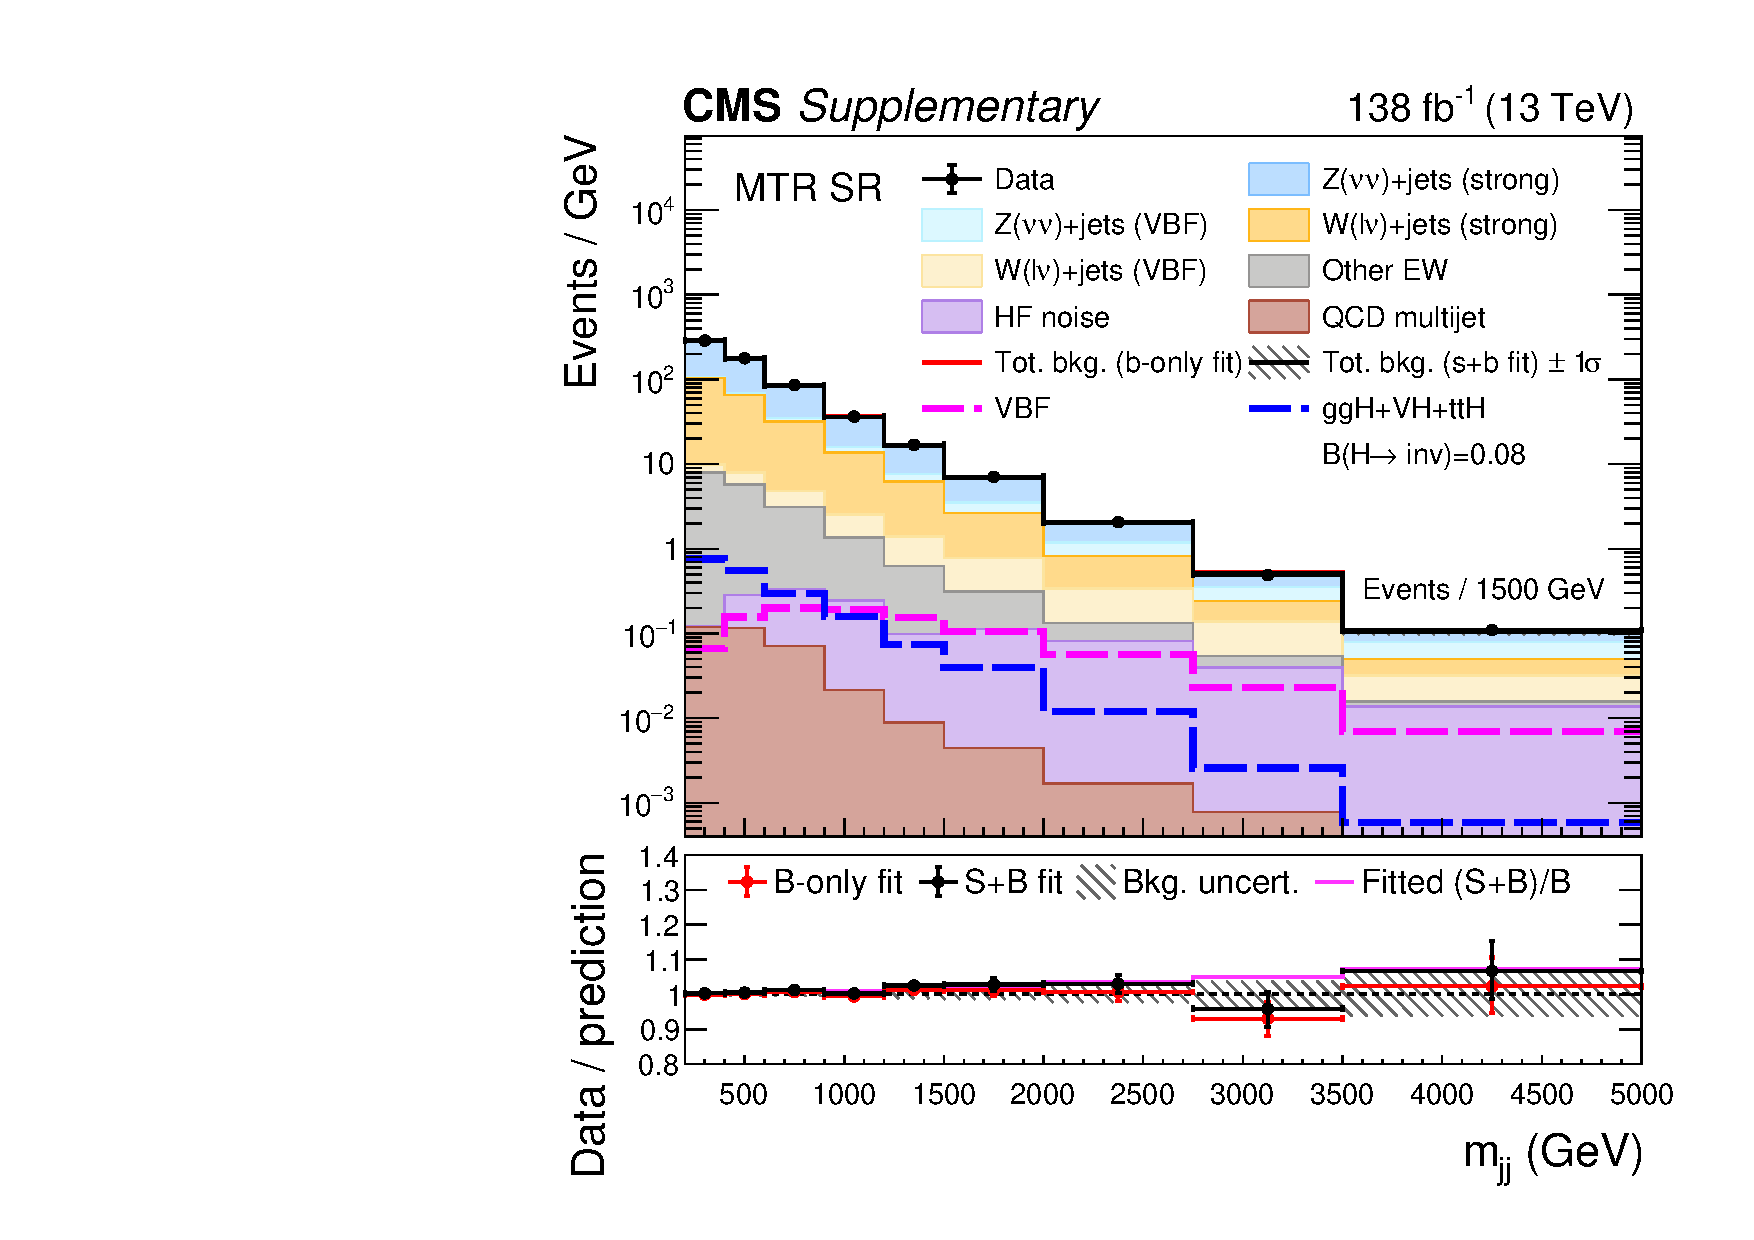
\includegraphics[width=0.7\textwidth]{\combPlotDir/SignalRegion_MTR_AllYears.pdf}
    \caption{The observed $\mjj$ distribution in the VBF signal region compared to the postfit backgrounds, with the 
    2016, 2017, and 2018 datasets. The signal processes are scaled by the fitted value of $\brinv$, shown in the legend. 
    The background contributions are estimated from 
    the fit to the data described in Sec.~\ref{subsec:likelihood_fit} (S+B fit). 
    The total background estimated from a fit assuming $\brinv=0$ (B-only fit) is also shown. 
    The last bin of each distribution sums events above the bin threshold divided by the bin width. Figure taken from~\cite{VBFHinvAnalysisPaper}.}
    \label{fig:mtr_comb_with_2016}
\end{figure}

\begin{table*}[htbp]
    \centering
    \caption{Uncertainty breakdown in $\brinv$. 
    The sources of uncertainty are separated into different groups. 
    Observed and expected results are quoted for the full combination of 2016, 2017, and 2018 data. 
    The expected results are obtained using an Asimov dataset~\cite{Cowan:2010js} with $\brhinv=0$.}
    \label{tab:uncertainty_scans}
    \cmsTable{
    \renewcommand{\arraystretch}{1.2} % Increase the row height by 20%
    \begin{tabular}{l c c}
       \hline
       Group of systematic uncertainties & Observed impact on \brinv & Expected impact on \brinv \\
      \hline
      Theory                & $^{+ 0.026}_{-0.025}$ & $\pm 0.024$ \\
      MC event count        & $^{+ 0.024}_{-0.023}$ & $^{+ 0.023}_{-0.024}$ \\
      Triggers              & $^{+ 0.021}_{-0.022}$ & $\pm 0.021$ \\
      Leptons/photons/b     & $^{+ 0.012}_{-0.011}$ & $^{+ 0.010}_{-0.011}$ \\
      QCD multijet mismodelling & $\pm 0.013$ & $\pm 0.014$ \\
      Jet calibration       & $^{+ 0.010}_{-0.007}$ & $\pm 0.007$ \\
      Int. luminosity/pileup & $\pm 0.005$ & $^{+ 0.004}_{-0.005}$ \\
      Other systematic uncertainties & $^{+ 0.013}_{-0.010}$ & $\pm 0.010$ \\
      \hline
      Stat.  & $\pm 0.029 $ & $\pm 0.030$ \\
      \hline
    \end{tabular}
     }
\end{table*}

From Fig.~\ref{fig:mtr_comb_with_2016}, it can be observed that no significant
excess of data is observed compared to the Standard Model background. Therefore, the results from this
analysis are interpreted as an upper bound on $\mu = \sigmabr$, the methodology and resulting upper bounds are 
described in the next section.

\clearpage